\cleardoublepage
\chapter{Tests, Results and Analysis}\label{chap:Tests}
% To do: 
% Color Scheme
% Red - Not started
% Yellow - In progress
% Blue - Done, under approval
% Green - Done and approved
\todo[inline,color=red!40]{*Chapter Introduction}
\todo[inline,color=red!40]{*1 - Software Tests}
\todo[inline,color=red!40]{*2 - Microphone Results}
\todo[inline,color=red!40]{*3 - Accelerometer and PiezoElectric Results}
%% Writing %%%%%%%%%%%%%%%%%%%%%%%%%%%%%%%%%%%%%%%%%%%%%%%%%%%%%%%%%%%%
\section{Algorithm Test}
The purpose of this test is to test the effectiveness of the algorithm implementation mentioned in~\ref{subsec:fftImp}, one way to perform this test is recurring to random signals with known frequencies, this way is possible to compare the results from the implementation in a microcontroller environment with the absolute frequency determined when generation the random signal.

To try to perform the tests as close as possible to the type of signals that were expected to obtain, several aspects were taken into consideration, for that reason a small explanation of how the signals were generated will be given. 
%----------------Introduction above this line--------------------------
\subsection{Signal Generation}\label{subsec:sigGen}
To try to synthetize a wave form as similar as possible to the one resulting from the work of~\citeauthor{wuLiquidLevelDetector2014b} in figure~\ref{fig:realsignalWu}.
\begin{figure}[]
    \centering
    \begin{subfigure}{0.45\textwidth}
        \centering
        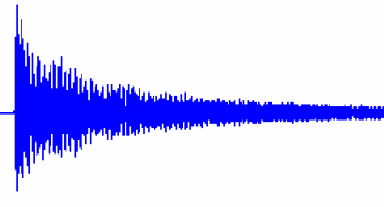
\includegraphics[width=\linewidth]{Chapters/6CHP/Figures/completesignalWu.pdf}
        \caption{Complete Signal}{}
        %\label{subfig:g1lines}
    \end{subfigure}
    \begin{subfigure}{0.45\textwidth}
        \centering
        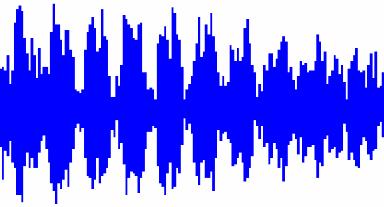
\includegraphics[width=\linewidth]{Chapters/6CHP/Figures/fractionWu.pdf}
        \caption{Fraction of the signal}{}
        %\label{subfig:g2lines}
    \end{subfigure}
    \caption{Real signal}{~\cite{wuLiquidLevelDetector2014b}}
     \label{fig:realsignalWu}
 \end{figure}
First is randomly define a frequency to be the dominant and a regular wave was generated, to create the decay effect the resulting wave is multiplied by $\frac{1}{e^{x}}$ being $x=1$, creating the echo effect by adding the original wave multiplied by the same equation, increasing the value of $x$ and adding the wave to the original shifting N/16, with N being the original size of the wave. This procedure is repeated to generate more waves with different frequencies and smaller amplitudes in the and random noise is added with random variance, being at maximum half of the previous wave. A example of the resulting waves can be observed in the figure~\ref{fig:synthetizedSignal}.
\begin{figure}[]
    \centering
    \begin{subfigure}{0.45\textwidth}
        \centering
        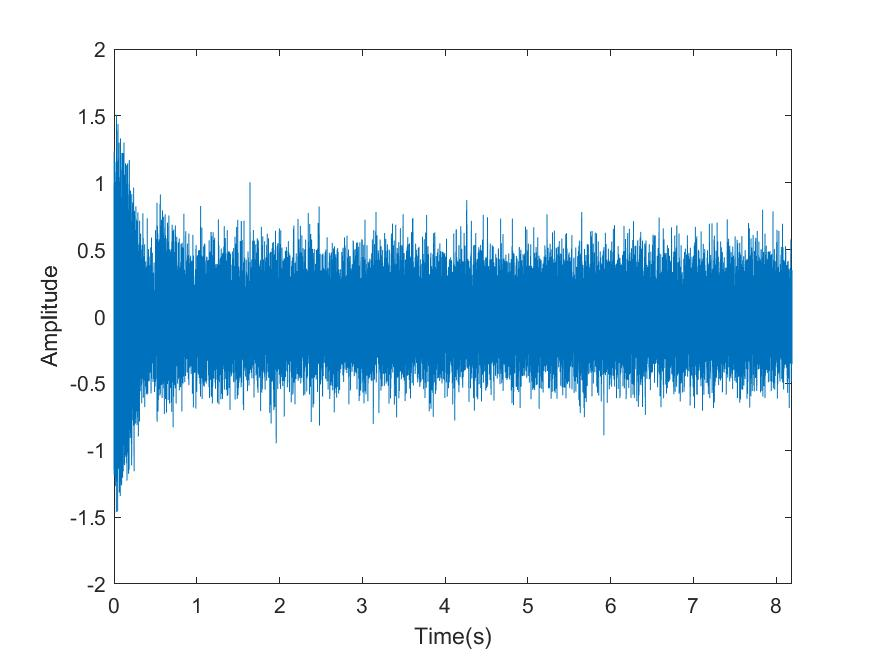
\includegraphics[width=\linewidth]{Chapters/6CHP/Figures/signal1.jpg}
        \caption{Noise variance of 0.05}{}
        %\label{subfig:g1lines}
    \end{subfigure}
    \begin{subfigure}{0.45\textwidth}
        \centering
        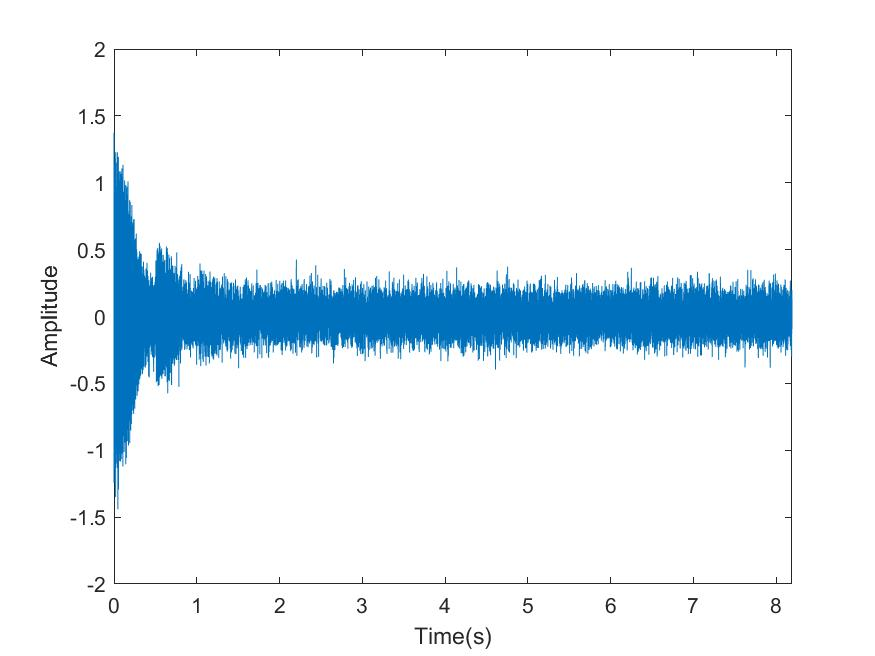
\includegraphics[width=\linewidth]{Chapters/6CHP/Figures/signal2.jpg}
        \caption{Noise variance of 0.01}{}
        %\label{subfig:g2lines}
    \end{subfigure}
    \begin{subfigure}{0.45\textwidth}
        \centering
        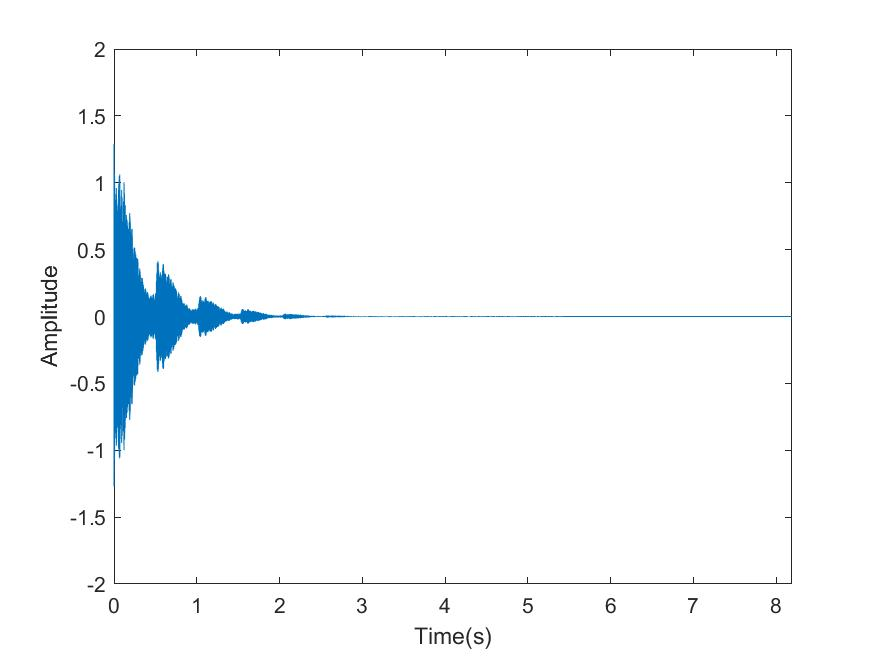
\includegraphics[width=\linewidth]{Chapters/6CHP/Figures/signal3.jpg}
        \caption{Noise variance of 0}{}
        %\label{subfig:g1lines}
    \end{subfigure}
    \begin{subfigure}{0.45\textwidth}
        \centering
        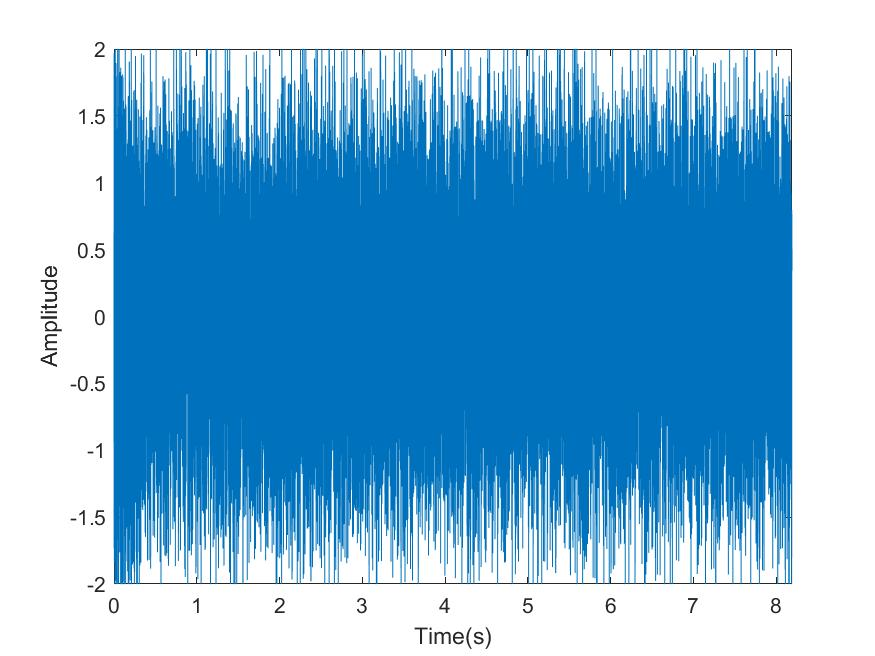
\includegraphics[width=\linewidth]{Chapters/6CHP/Figures/signal4.jpg}
        \caption{Noise variance of 0.5}{}
        %\label{subfig:g2lines}
    \end{subfigure}
    \caption{Example of signals synthetized with MatLab with different noise variances}{}
     \label{fig:synthetizedSignal}
 \end{figure}
\subsection{Tests}
To tests the effectiveness of the FFT algorithm in use, were perform in total 1000 tests to verify the obtained error of the implementation. The tests weren't only performed to the Fixed-Point algorithm in the microcontroller, the same code used in the microcontroller was also implemented in a PC and the FFT function of MATLAB was used as a control test, to verify that the signal wasn't to corrupted with noise that even MATLAB wasn't able to determine the dominant frequency correctly.

In a PC environment was implemented both FFTs, the Fixed-Point and the Floating-Point, in the microcontroller it was only possible to perform tests with the Fixed-Point since the other version exceeded the amount of memory needed to use the implementation. In each test a random signal was generated, as mentioned in~\ref{subsec:sigGen}, 512 samples of that signal were selected and converted to values between 0 and 1023, just like if it was converted by an ADC. After generating the signal, the dominant frequency is saved, to compare with the results, the samples are processed in MATLAB and a dominant frequency is obtained and saved as well. The samples used in MATLAB environment are saved, in order to be tested in both implementation in the PC environment and the obtained results are saved, to finalize the samples are sent to the microcontroller and processed and the result is sent back to the PC and saved. After all the tests, the results obtained are compared with the original value used in the frequency, allowing to verify how the algorithm performs. 
\begin{figure}[]
    \centering
    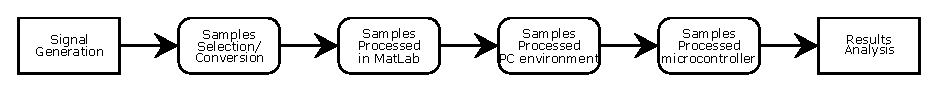
\includegraphics[width=1\textwidth]{Chapters/6CHP/Figures/ProcFlow.eps}
    \caption{Flow of signal processing in different environments}{}
    \label{fig:flowProc}
\end{figure}
Although the tests were perform in other environments, the test that is the most important is the one in the microcontroller. In the tests performed in the microcontroller not only the validity of the implementation, but is also necessary how long it takes to execute the algorithm in the microcontroller and what are the memory needs of the program. The program that executes the algorithm was built to start measuring the execution time of the FFT implementation right before it starts, and end it after calculated the magnitude of the resulting signal, to measure how long takes to perform these tasks it uses one of the timers that the microcontroller has. To better understand how all works, observe figure\ref{fig:dataProcuC}.
\begin{figure}[]
    \centering
    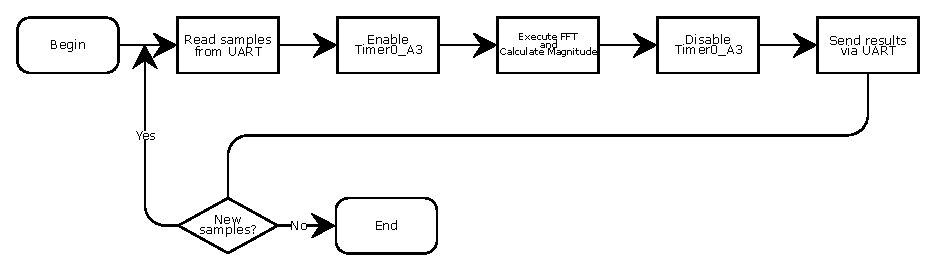
\includegraphics[width=1\textwidth]{Chapters/6CHP/Figures/uCDataProc.eps}
    \caption{Flow of signal processing in different environments}{}
    \label{fig:dataProcuC}
\end{figure}
\subsection{Results}
The resulting data obtained is the dominant frequency of each implementation with the FFT, additionally in the microcontroller option was also measured the execution time of the algorithm. In the resulting dominant frequency from all cases was then compared with the absolute frequency, that was saved every time that a new signal was generated, the error obtained in each implementation ca be observer in the table~\ref{tab:perfRes}.
\begin{table}
    \centering
    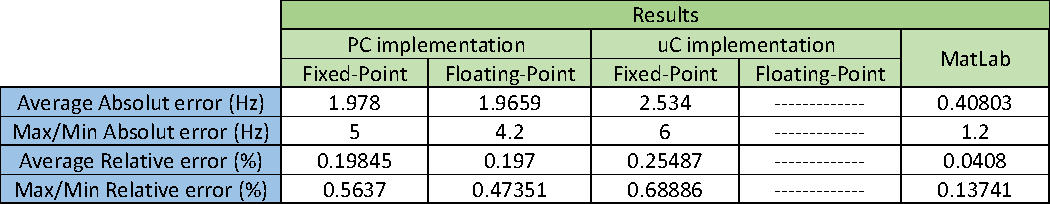
\includegraphics[width=1\textwidth]{Chapters/6CHP/Figures/performanceAlgorithm.pdf}
    \caption{Results of the execution of a synthetic signal in the different algorithms}
    \label{tab:perfRes}
\end{table}
Is evident that the results from MATLAB are much better when compared with the rest and when comparing the Floating-Point with the Fixed-Point, in the PC results, there is a slight difference between the two, but for the microcontroller in use wasn't possible to implement the Floating-Point, anyway the error obtained in the Fixed-Point doesn't increase significativily, with these results the use of the algorithm ca be used with no problems, still quite precise for the application that will be used. The results of the execution time of the algorithm ca be observed in table~\ref{tab:excTimeuC}, the number of ticks is due the fact that to measure the execution time, a timer was configured with to generate an interruption every 500$\mu$s, incrementing a variable each time that happen, as a results multiplying the number of ticks by the time each interruption is generated gives the execution time of the algorithm. Taking into consideration that is microcontroller with a small processing power and the embedded Hardware Multiplier hasn't been used, around 3s to process 512 samples is acceptable, since isn't mandatory to the results being in real time.  
\begin{table}
    \centering
    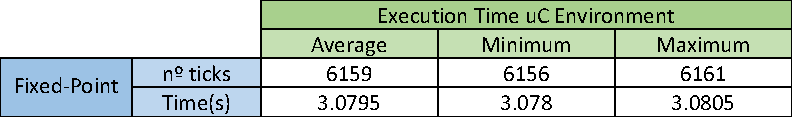
\includegraphics[width=1\textwidth]{Chapters/6CHP/Figures/excTimeuC.pdf}
    \caption{Results of the execution of the Fixed-Point implementation in the microcontroller}
    \label{tab:excTimeuC}
\end{table}

\section{Microphone Results}
\section{Accelerometer and PiezoElectric Results}


\clearpage
%\printbibliography[heading=subbibliography]
%\addcontentsline{toc}{section}{References}